%! @@TITLE@@ — Unit @@UNITINT@@, Lesson @@LESSONID@@ — Guided Notes & Practice
% THE in-class document, in the MAIN IDEAS / NOTES shape (LESSON_SHAPE.md §1): the vocabulary
% box, then ONE two-column guidednotes table. Each row is one idea — a label on the left; on the
% right one or two COMPLETE printed sentences, ONE large pre-drawn display, then a two-across
% grid of a few numbered problems with 2–3cm of writing room. Problems run 1..N (aim 12–19).
% DENSITY: the page belongs to the student's pen. A \blank{} only where a word or number IS the
% answer (a table to fill, a display to name) — never mid-sentence. Short printed text, big
% pictures, big answer spaces. 3–4 pages.
%   I DO   : the teacher reads the definition, marks up the display, works the first problem.
%   WE DO  : the class works the rest of each grid, students holding the pen; the last row,
%            Guided Practice, is worked entirely together in a fresh context.
%   YOU DO : nothing on this page — ../homework/ IS the individual practice. No independent
%            set, no reflection box, no objectives box (targets are on the cover).
% The crux — the problem that surfaces the target misconception — is in the grid of the LAST
% INSTRUCTION ROW, before Guided Practice.
%
% PAGE LOCKSTEP with notes_key/: \termblank -> \termans, \blank -> \ans, and the answer argument
% of every \pcell, \writespace and \labelbox filled. Nothing else differs. Answer spaces are
% fixed heights, so the two files cannot drift.
% TABLE MECHANICS: inside a cell, `\\` ENDS THE ROW — break lines with \par. A row cannot break
% across pages: the figure gets its own sub-row (`\\` then `& ...`) and EACH GRID ROW is its own
% sub-row — close the probgrid, `\\ &`, reopen as probgrid* (no top rule).
% NO SKETCH QUESTIONS: every display is pre-drawn in TikZ and read.
\documentclass[12pt]{article}
\usepackage{@@PREFIX@@-article}
\usepackage{@@PREFIX@@-boxes}
% Vocabulary rows: copy the \vterm / \vtermans block from unit01/lesson02/notes/main.tex
% (fixed-height rows, no rule line — user correction 2026-09-06). \wordbank only above a fill table.

\begin{document}

\pageheader{Unit @@UNITINT@@, Lesson @@LESSONID@@}{Guided Notes \& Practice}
% NAMESTRIP: no \namedateperiod here — the name row lives on the cover only.

\vspace{2pt}

% ── VOCABULARY (I do — students fill each term AS IT IS NAMED, never in advance) ──
\boxguard[16]
\begin{vocabbox}
\small
Fill in each term \textbf{as we name it} in the notes below.
\par
\vterm{TODO Term 1}
\par
\vterm{TODO Term 2}
\par
\vterm{TODO Term 3}
\par
\end{vocabbox}

% ── HOOK (stays — the 60-second context whose numbers the rows below reuse) ──
\boxguard[14]
\begin{hookbox}
\small
TODO: the hook, two or three sentences, and one question left hanging.
\par\writelines{2}
\end{hookbox}

\small
\begin{guidednotes}
% ── ROW 1: TODO idea ─────────────────────────────────────────────────────────
\mainidea[TODO lead]{TODO Label} &
TODO: one or two complete sentences. A \textbf{TODO term} is TODO. \textbf{The test:} TODO.

\vspace{4pt}
\begin{center}
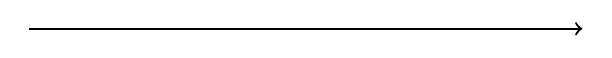
\begin{tikzpicture}[scale=0.95]
  % TODO: a large pre-drawn display that SHOWS the idea
  \draw[->, thick] (-0.2,0) -- (7.2,0);
\end{tikzpicture}
\end{center}
\\
& \notesprompt{TODO Classify each \dots\ Say how you know.}
\begin{probgrid}{|Y|Y|}
\pcell{1}{TODO}{2.0cm}{} & \pcell{2}{TODO}{2.0cm}{} \\ \hline
\end{probgrid}
\\
& \begin{probgrid}*{|Y|Y|}
\pcell{3}{TODO --- the trap}{2.0cm}{} & \pcell{4}{TODO}{2.0cm}{} \\ \hline
\end{probgrid}
\\ \hline
% ── ROW 2: TODO idea with a display to annotate ──────────────────────────────
\mainidea[TODO lead]{TODO Label} &
TODO: the context in one sentence. \textbf{TODO: the one thing to notice.}

\vspace{4pt}
\begin{center}
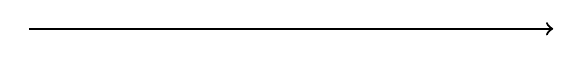
\begin{tikzpicture}[scale=0.9]
  % TODO: pre-drawn display
  \draw[->, thick] (-0.2,0) -- (7.2,0);
\end{tikzpicture}\\[6pt]
This is a \labelbox{2.4cm}{}
\end{center}
\\
& \notesprompt{Read it.}
\begin{probgrid}{|Y|Y|}
\pcell{5}{TODO}{1.8cm}{} & \pcell{6}{TODO}{1.8cm}{} \\ \hline
\end{probgrid}
\\
& \begin{probgrid}*{|Y|Y|}
\pcell{7}{TODO}{1.8cm}{} & \pcell{8}{\textbf{In your own words:} TODO}{1.8cm}{} \\ \hline
\end{probgrid}
\\ \hline
% ── ROW 3: TODO procedure ────────────────────────────────────────────────────
\mainidea{TODO Label} &
TODO: the setup sentence.

\vspace{3pt}
\stepnum{1}\ TODO step.\par
\stepnum{2}\ TODO step.\par
\stepnum{3}\ TODO step.

\vspace{5pt}
\textbf{9.} TODO: a table the student fills (its cells are the only \blank{}s on the page).
\\
& \begin{center}
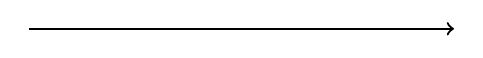
\begin{tikzpicture}[scale=0.9]
  % TODO: the display the procedure produces, pre-drawn
  \draw[->, thick] (0,0) -- (6,0);
\end{tikzpicture}
\end{center}
\\
& \textbf{TODO: the sentence to land.}
\notesprompt{Use it.}
\begin{probgrid}{|Y|Y|}
\pcell{10}{TODO}{2.2cm}{} & \pcell{11}{TODO}{2.2cm}{} \\ \hline
\end{probgrid}
\\ \hline
% ── ROW 4: THE CRUX — the target misconception as problems in a grid ─────────
\mainidea[TODO lead]{TODO Label} &
TODO: the contrast, in one sentence.

\vspace{2pt}
\begin{center}
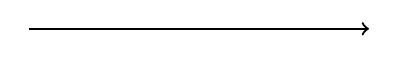
\begin{tikzpicture}[scale=0.72]
  % TODO: the two pictures side by side
  \draw[->, thick] (0,0) -- (6,0);
\end{tikzpicture}
\end{center}
\\
& \fcolorbox{cerulean}{frost}{\parbox{\dimexpr\linewidth-2\fboxsep-2\fboxrule\relax}{\centering
\textbf{TODO: the sentence to land, printed whole.}}}

\vspace{3pt}
\textbf{In your own words:} TODO the question that makes them restate it.
\writespace{1.6cm}{}
\\
& \notesprompt{TODO Compare.}
\begin{probgrid}{|Y|Y|}
\pcell{12}{TODO}{2.4cm}{} & \pcell{13}{TODO}{2.4cm}{} \\ \hline
\end{probgrid}
\\
& \begin{probgrid}*{|Y|Y|}
\pcell{14}{TODO --- the crux}{2.4cm}{} & \pcell{15}{TODO --- the counterweight}{2.4cm}{} \\ \hline
\end{probgrid}
\\ \hline
% ── LAST ROW: GUIDED PRACTICE — we do, together, a fresh context ─────────────
\mainidea[Guided practice]{TODO Title} &
TODO: the fresh context in one sentence.

\vspace{2pt}
\begin{center}
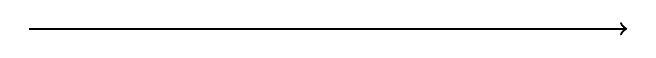
\begin{tikzpicture}[scale=1.0]
  % TODO: its pre-drawn display
  \draw[->, thick] (-0.2,0) -- (7.4,0);
\end{tikzpicture}
\end{center}
\\
& \notesprompt{We work these together.}
\begin{probgrid}{|Y|Y|}
\pcell{16}{TODO}{2.2cm}{} & \pcell{17}{TODO}{2.2cm}{} \\ \hline
\end{probgrid}
\\
& \begin{probgrid}*{|Y|Y|}
\pcell{18}{TODO --- the crux transferred}{2.6cm}{} & \pcell{19}{TODO}{2.6cm}{} \\ \hline
\end{probgrid}
\\ \hline
\end{guidednotes}

% ── THE NOTES END AT GUIDED PRACTICE ─────────────────────────────────────────
% There is deliberately no "you do" here: ../homework/ is the individual practice,
% started in class in the last 8 minutes while the teacher circulates.

\end{document}
